\documentclass{article}\usepackage[]{graphicx}\usepackage[]{color}
%% maxwidth is the original width if it is less than linewidth
%% otherwise use linewidth (to make sure the graphics do not exceed the margin)
\makeatletter
\def\maxwidth{ %
  \ifdim\Gin@nat@width>\linewidth
    \linewidth
  \else
    \Gin@nat@width
  \fi
}
\makeatother

\definecolor{fgcolor}{rgb}{0.345, 0.345, 0.345}
\newcommand{\hlnum}[1]{\textcolor[rgb]{0.686,0.059,0.569}{#1}}%
\newcommand{\hlstr}[1]{\textcolor[rgb]{0.192,0.494,0.8}{#1}}%
\newcommand{\hlcom}[1]{\textcolor[rgb]{0.678,0.584,0.686}{\textit{#1}}}%
\newcommand{\hlopt}[1]{\textcolor[rgb]{0,0,0}{#1}}%
\newcommand{\hlstd}[1]{\textcolor[rgb]{0.345,0.345,0.345}{#1}}%
\newcommand{\hlkwa}[1]{\textcolor[rgb]{0.161,0.373,0.58}{\textbf{#1}}}%
\newcommand{\hlkwb}[1]{\textcolor[rgb]{0.69,0.353,0.396}{#1}}%
\newcommand{\hlkwc}[1]{\textcolor[rgb]{0.333,0.667,0.333}{#1}}%
\newcommand{\hlkwd}[1]{\textcolor[rgb]{0.737,0.353,0.396}{\textbf{#1}}}%
\let\hlipl\hlkwb

\usepackage{framed}
\makeatletter
\newenvironment{kframe}{%
 \def\at@end@of@kframe{}%
 \ifinner\ifhmode%
  \def\at@end@of@kframe{\end{minipage}}%
  \begin{minipage}{\columnwidth}%
 \fi\fi%
 \def\FrameCommand##1{\hskip\@totalleftmargin \hskip-\fboxsep
 \colorbox{shadecolor}{##1}\hskip-\fboxsep
     % There is no \\@totalrightmargin, so:
     \hskip-\linewidth \hskip-\@totalleftmargin \hskip\columnwidth}%
 \MakeFramed {\advance\hsize-\width
   \@totalleftmargin\z@ \linewidth\hsize
   \@setminipage}}%
 {\par\unskip\endMakeFramed%
 \at@end@of@kframe}
\makeatother

\definecolor{shadecolor}{rgb}{.97, .97, .97}
\definecolor{messagecolor}{rgb}{0, 0, 0}
\definecolor{warningcolor}{rgb}{1, 0, 1}
\definecolor{errorcolor}{rgb}{1, 0, 0}
\newenvironment{knitrout}{}{} % an empty environment to be redefined in TeX

\usepackage{alltt}
\usepackage{natbib}
\IfFileExists{upquote.sty}{\usepackage{upquote}}{}
\begin{document}





\title{The Masque of the Red Death by Edgar Allan Poe Wordcloud}
\author{Dayana Moncada}
\maketitle

\begin{abstract}
In this article we construct a wordcloud, using the tidytext R package, for Edgar A. Poe's The Masque of the Red Death novel. 

\end{abstract}

\textit{The Masque of the Red Death} 
"The Masque of the Red Death", originally published as "The Mask of the Red Death: A Fantasy" (1842), is a short story by Edgar Allan Poe. The story follows Prince Prospero's attempts to avoid a dangerous plague, known as the Red Death, by hiding in his abbey. He, along with many other wealthy nobles, hosts a masquerade ball within seven rooms of the abbey, each decorated with a different color. In the midst of their revelry, a mysterious figure disguised as a Red Death victim enters and makes his way through each of the rooms. Prospero dies after confronting this stranger, whose "costume" proves to contain nothing tangible inside it; the guests also die in turn

\section{The gutenbergr Package} 
Download and process public domain works in the Project Gutenberg collection http://www.gutenberg.org/. Includes metadata for all Project Gutenberg works, so that they can be searched and retrieved.

\begin{knitrout}
\definecolor{shadecolor}{rgb}{0.969, 0.969, 0.969}\color{fgcolor}\begin{kframe}
\begin{alltt}
\hlkwd{library}\hlstd{(gutenbergr)}
\hlkwd{gutenberg_works}\hlstd{(author} \hlopt{==} \hlstr{"Poe, Edgar Allan"}\hlstd{)}
\end{alltt}
\begin{verbatim}
## # A tibble: 16 x 8
##    gutenberg_id
##           <int>
##  1          932
##  2         1062
##  3         1063
##  4         1064
##  5         1065
##  6         2147
##  7         2148
##  8         2149
##  9         2150
## 10         2151
## 11         8893
## 12        10031
## 13        25525
## 14        32037
## 15        45484
## 16        50852
## # ... with 7 more variables: title <chr>, author <chr>,
## #   gutenberg_author_id <int>, language <chr>, gutenberg_bookshelf <chr>,
## #   rights <chr>, has_text <lgl>
\end{verbatim}
\begin{alltt}
\hlstd{poe}\hlkwb{<-}\hlkwd{gutenberg_download}\hlstd{(}\hlnum{1064}\hlstd{)}
\end{alltt}
\end{kframe}
\end{knitrout}


\noindent Now we are ready for some data cleaning.

\section{The Wordcloud}
To make the wordcloud, we first have to break up the lines into words.  We can use a function from the tidytext package for this:

\begin{knitrout}
\definecolor{shadecolor}{rgb}{0.969, 0.969, 0.969}\color{fgcolor}\begin{kframe}
\begin{alltt}
\hlkwd{library}\hlstd{(dplyr)}
\hlkwd{library}\hlstd{(tidytext)}
\hlstd{poe_words}\hlkwb{<-}\hlstd{poe}\hlopt
  \hlkwd{unnest_tokens}\hlstd{(word,text)}
\end{alltt}
\end{kframe}
\end{knitrout}

We can remove common, unimportant words with the stop\_words data frame and some dplyr:
\begin{knitrout}
\definecolor{shadecolor}{rgb}{0.969, 0.969, 0.969}\color{fgcolor}\begin{kframe}
\begin{alltt}
\hlstd{poe_words}\hlkwb{<-}\hlstd{poe_words}\hlopt
  \hlkwd{filter}\hlstd{(}\hlopt{!}\hlstd{(word} \hlopt \hlstd{stop_words}\hlopt{$}\hlstd{word))}

\hlstd{poe_words}
\end{alltt}
\begin{verbatim}
## # A tibble: 921 x 2
##    gutenberg_id       word
##           <int>      <chr>
##  1         1064     masque
##  2         1064        red
##  3         1064      death
##  4         1064      edgar
##  5         1064      allan
##  6         1064        poe
##  7         1064        red
##  8         1064      death
##  9         1064 devastated
## 10         1064    country
## # ... with 911 more rows
\end{verbatim}
\end{kframe}
\end{knitrout}


Now, we need to calculate the frequencies of the words in the novel.  Again, we can use standard dplyr techniques for this:
\begin{knitrout}
\definecolor{shadecolor}{rgb}{0.969, 0.969, 0.969}\color{fgcolor}\begin{kframe}
\begin{alltt}
\hlkwd{library}\hlstd{(dplyr)}
\hlstd{poe_freq}\hlkwb{<-}\hlstd{poe_words}\hlopt
  \hlkwd{group_by}\hlstd{(word)}\hlopt
  \hlkwd{summarize}\hlstd{(}\hlkwc{count}\hlstd{=}\hlkwd{n}\hlstd{())}
\end{alltt}
\end{kframe}
\end{knitrout}

Finally, it's time to generate the wordcloud:
\begin{knitrout}
\definecolor{shadecolor}{rgb}{0.969, 0.969, 0.969}\color{fgcolor}\begin{kframe}
\begin{alltt}
\hlkwd{library}\hlstd{(wordcloud)}
\hlkwd{wordcloud}\hlstd{(poe_freq}\hlopt{$}\hlstd{word,poe_freq}\hlopt{$}\hlstd{count)}
\end{alltt}
\end{kframe}
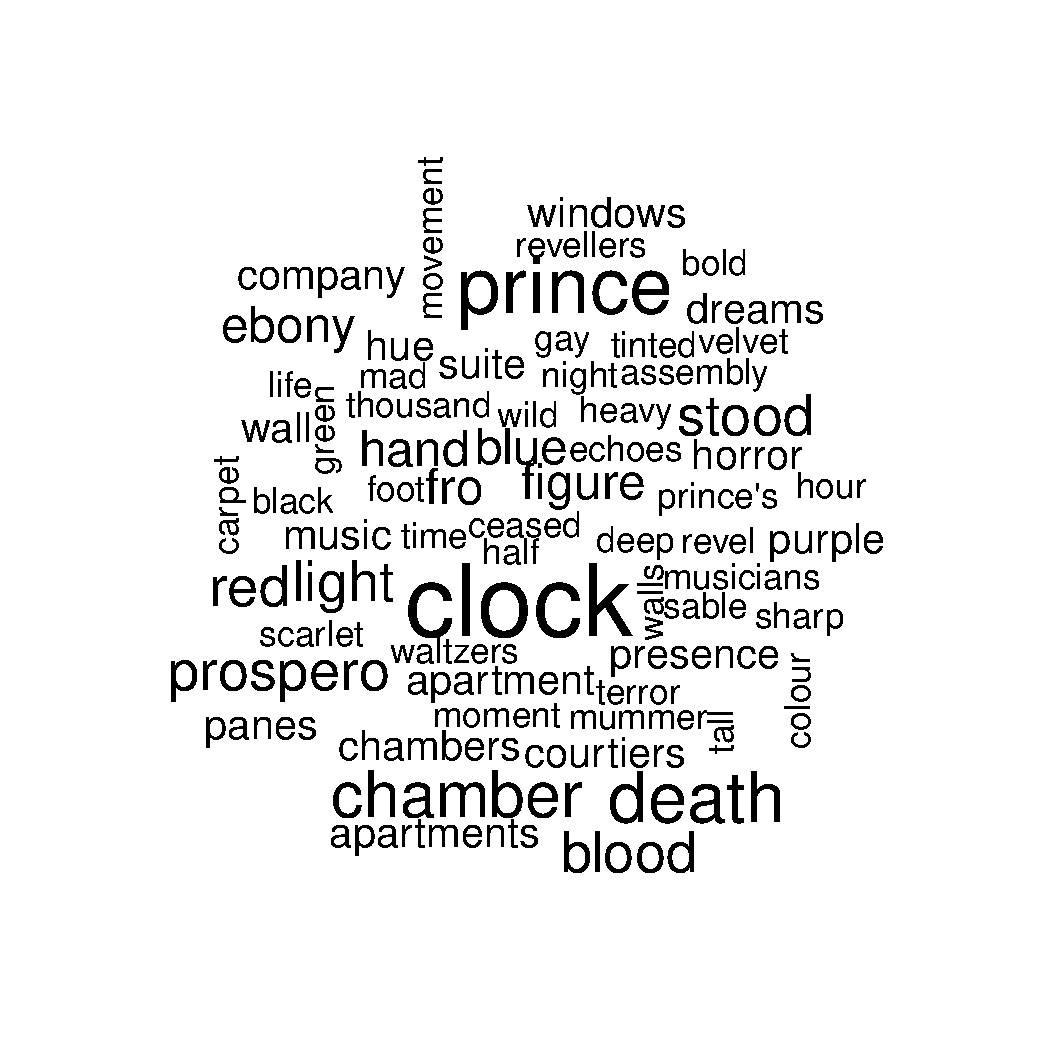
\includegraphics[width=\maxwidth]{figure/unnamed-chunk-6-1} 

\end{knitrout}

\bibliographystyle{apa}
\bibliography{article,packages}
\nocite{*}


\end{document}
